% ======================================================================
%  Conformal Crop Classification Across Regions with Sentinel-2
%  IEEE conference draft (shared core for AI2ML 2026 / ICoDT2)
%  Build: pdflatex main && bibtex main && pdflatex main && pdflatex main
% ======================================================================
\documentclass[conference]{IEEEtran}
\IEEEoverridecommandlockouts
% The preceding line is only needed to identify funding in the first footnote.
% Packages below follow conference_101719.tex; algorithmic is omitted (no
% algorithm floats), and booktabs/array/url/stfloats are the only additions.
\usepackage{cite}
\usepackage{amsmath,amssymb,amsfonts}
\usepackage{graphicx}
\usepackage{textcomp}
\usepackage{xcolor}
\usepackage{booktabs}
\usepackage{array}
\usepackage{url}
\usepackage{stfloats}   % allow full-width figure*/table* to place at column bottoms too
\usepackage{microtype}  % protrusion + expansion: fewer loose lines and orphan words

% Tighten float/text separation. IEEEtran defaults are 1.55\baselineskip for
% \textfloatsep and \dbltextfloatsep and 0.85\baselineskip for the rest; the
% dbl* lengths matter here because two figures span both columns.
\setlength{\textfloatsep}{6pt plus 1pt minus 1pt}
\setlength{\intextsep}{6pt plus 1pt minus 1pt}
\setlength{\dbltextfloatsep}{6pt plus 1pt minus 1pt}
\setlength{\floatsep}{6pt plus 1pt minus 1pt}
\setlength{\dblfloatsep}{6pt plus 1pt minus 1pt}

\begin{document}

\title{Conformal Crop Classification Across Regions with Sentinel-2 Time Series}

% Three author blocks on the first row, the fourth centred on a second row.
% In conference mode \and is \end{@IEEEauthorhalign}<sep>\begin{@IEEEauthorhalign}
% and the author area is a centred paragraph, so the optional argument of \and
% is the supported place to close one row and open the next.
\author{\IEEEauthorblockN{Rao Muhammad Saeed Ali}
\IEEEauthorblockA{\textit{National University of Sciences} \\
\textit{and Technology (NUST)} \\
Islamabad, Pakistan \\
rali.msai23seecs@seecs.edu.pk}
\and
\IEEEauthorblockN{Muhammad Moazam Fraz}
\IEEEauthorblockA{\textit{National University of Sciences} \\
\textit{and Technology (NUST)} \\
Islamabad, Pakistan \\
moazam.fraz@seecs.edu.pk}
\and
\IEEEauthorblockN{Sami Ullah}
\IEEEauthorblockA{\textit{University of Birmingham} \\
Birmingham, United Kingdom \\
s.ullah@bham.ac.uk}
\and[{\hfill\mbox{}\\[1.2em]\mbox{}\hfill}]
\IEEEauthorblockN{Zuhair Zafar}
\IEEEauthorblockA{\textit{National University of Sciences} \\
\textit{and Technology (NUST)} \\
Islamabad, Pakistan \\
zuhair.zafar@seecs.edu.pk}}

% Copyright notice on the bottom of page 1. Must precede \maketitle, and needs
% the \IEEEoverridecommandlockouts above, since conference mode locks \IEEEpubid out.
\IEEEpubid{\makebox[\columnwidth]{979-8-3195-0250-6/26/\$31.00~\copyright2026
IEEE\hfill}\hspace{\columnsep}\makebox[\columnwidth]{}}

\maketitle

\begin{abstract}
Deep classifiers for satellite image time series (SITS) report near-perfect crop-type
accuracy, but those figures come from random cross-validation, which leaks spatially
correlated parcels and guarantees nothing for the unseen regions where a map is
deployed. Crop classification in Pakistan (85{,}618 fields, 79 districts, two seasons)
is studied here under a spatial protocol pairing district-grouped cross-validation
with a spatially disjoint test set. Conformal prediction then exposes the geographic
coverage gap. Split conformal keeps its target coverage on average under shift, at
about 0.89, while its per-region variance explodes. It therefore holds marginally and
fails conditionally, missing the target in up to 28\% of held-out regions and
collapsing to 0.68 in the worst. The gap holds across all eight backbones tested, making it a
property of spatially structured geospatial learning rather than of any model. A
region-robust threshold restores overall coverage and a class-conditional variant
restores per-crop coverage, but under a long tail the latter is bought with
near-vacuous sets for the very classes it should protect. Holding out whole provinces
shows the remedy transferring to a larger shift only once its safety margin is widened
beyond the district-tuned value. All results come from one country and one cropping
year, so the claims are for spatial transfer within that setting.
\end{abstract}

\begin{IEEEkeywords}
conformal prediction, uncertainty quantification, distribution shift, domain
generalization, spatial cross-validation, trustworthy machine learning, crop-type
mapping, satellite image time series, Sentinel-2.
\end{IEEEkeywords}

% ======================================================================
\section{Introduction}
% ======================================================================
Crop-type maps guide food-security monitoring, subsidy allocation, and agricultural
planning, and the stakes are highest in farming economies such as Pakistan.
Sentinel-2 has made deep learning on satellite image time series (SITS) the standard
approach, with accuracy above 90\% now routinely
reported~\cite{pelletier2019tempcnn,garnot2020ltae,tarasiou2023tsvit}.

Two gaps separate those numbers from a working system. The first is optimistic
testing. Random cross-validation puts neighbouring fields in both the training and
test sets, and neighbours share soil, irrigation, and management, so accuracy is
inflated by spatial
autocorrelation~\cite{roberts2017cv,meyer2019spatialcv,ploton2020spatial}. The second
is reliability. A finished map is used in districts with no ground truth, where
someone still has to judge which fields to trust, and a raw softmax score carries no
guarantee.

Conformal prediction~\cite{vovk2005algorithmic,angelopoulos2023conformal} addresses
the second gap. Instead of a single label it returns a set of candidate labels, chosen
so that the set contains the true label a fixed fraction of the time, here 90\%. That
promise holds only if the calibration and test fields are alike, and moving to a new
region breaks it. The effect is easy to see. A predictor calibrated on surveyed fields
is asked to map a district it never saw, and its user is promised the true crop in 90
of every 100 sets. In the worst held-out district that figure is 68 in 100, and
nothing in the output flags it. Averaged over districts, coverage still reads 0.89 and
looks healthy. The promise holds on average and fails where the map is used. This is
the geographic coverage gap. No distribution-free method can promise coverage in every
region at once~\cite{barber2023nonexchangeable}, so the aim is to control the failure
rather than remove it.

Fitting a separate threshold in each region and taking a conservative quantile across
regions restores the overall promise, and repeating that within each crop restores it
crop by crop. The price is that rare crops then get sets holding nearly every
candidate, which are reliable but say little. Tighter sets, not more coverage, are
what is missing, so the backbone is also trained with a set-size
penalty~\cite{stutz2022conformal}.

This work makes four contributions. The first is a strict spatial protocol that
measures the optimism of random validation, released as a reusable testbed. The
second is the geographic coverage gap, present in all eight backbones tested, with
region-robust and class-conditional calibration that close it; holding out whole
provinces shows the district-tuned margin to be too small. The third is
conformal-efficiency-aware training, which tightens sets for the common crops but
hits a floor for the rarest. The fourth is a data-centric recipe built on symmetric
cross-entropy. Accuracy is saturated across architectures, so a compact state-space
model (PhenoSSM) suffices and the bottleneck is reliability, not capacity. All results
come from one country and one cropping year, so only spatial transfer is measured.

% ======================================================================
\section{Related Work}
% ======================================================================
Crop typing from SITS has progressed from random forests~\cite{roberts2017cv} through
temporal convolution~\cite{pelletier2019tempcnn} and temporal
self-attention~\cite{garnot2020ltae} to the transformers, foundation
models, and state-space models that now hold the accuracy
frontier on public benchmarks~\cite{tarasiou2023tsvit,tseng2024presto,gu2022s4d}.
Which of them leads matters less than it appears, since the results below show
accuracy saturating across architectures once validation is spatial. Almost all of
this work reports accuracy under random cross-validation. Geospatial samples are
spatially autocorrelated, so a random split places near-duplicate parcels in both
training and test and rewards memorisation over transfer~\cite{roberts2017cv}.
Spatial block and group cross-validation remove this
leakage~\cite{meyer2019spatialcv}, and audits have caught random splits overstating
skill by wide margins~\cite{ploton2020spatial}. Crop mapping has been slow to adopt
it, so the distance between reported accuracy and accuracy in an unseen district
remains largely uncharacterised. That distance is the first problem studied here.

Deployable maps additionally need actionable uncertainty. Temperature
scaling~\cite{guo2017calibration} and selective
classification~\cite{geifman2017selective} improve calibration or abstain on hard
inputs, but neither provides a coverage guarantee. Conformal
prediction~\cite{vovk2005algorithmic,angelopoulos2023conformal} does, returning label
sets that contain the truth with a user-specified probability through nonconformity
scores such as adaptive prediction sets~\cite{romano2020aps}. Its guarantee is only
marginal, and three separate lines
of work each strengthen one axis that a deployed crop map needs at once. Mondrian and
class-conditional constructions~\cite{ding2024longtailconformal} secure per-class
coverage for long tails, and weighted conformal corrects estimable covariate
shift~\cite{tibshirani2019covshift}. Non-exchangeable and distributionally robust
methods~\cite{barber2023nonexchangeable,cauchois2024robust} bound
coverage loss under shift, subject to the limit that distribution-free conditional
coverage over arbitrary regions is impossible~\cite{barber2023nonexchangeable}. Set
efficiency can be improved separately by conformal training~\cite{stutz2022conformal}.
In remote sensing, conformal prediction has reached only static land-cover
maps~\cite{singh2024conformallulc}, not crop time series, and the joint behaviour of
those three axes has not been studied. Characterising that interaction and its cost is
the central open problem here.

Survey-derived crop labels are, finally, both long-tailed and noisy, often on the same
fields. Focal loss~\cite{lin2017focal} and logit adjustment~\cite{menon2021logitadjust}
rebalance toward rare classes, while generalized and symmetric
cross-entropy~\cite{zhang2018gce,wang2019sce} and confident
learning~\cite{northcutt2021confident} guard against label
noise. Which helps when rarity and noise coincide is examined directly.

% ======================================================================
\section{Study Area and Data Analysis}\label{sec:data}
% ======================================================================
The ground truth is the Asian Development Bank crop-type survey of Pakistan, Rabi 2022
to Kharif 2023. It begins as 135{,}408 raw (field, season, crop) boundary polygons over
79 districts and two seasons, Rabi (October to April) and Kharif (May to November),
distributed as in Fig.~\ref{fig:spatial}. The task is field-level crop typing, one
label per delineated field. Monthly median composites are built from harmonised
Sentinel-2 surface reflectance with Scene Classification Layer cloud masking, monthly
because monsoon cloud during Kharif makes single-date acquisitions unreliable. Ten
spectral bands plus NDVI, EVI, NDWI, and SAVI are kept, each as its within-field mean
and standard deviation, giving a $T{=}7$ by $C{=}28$ tensor per field. Each index is
formed per pixel and only then averaged, so the index channels are not recoverable
from the band means, though a feature ablation shows them to be accuracy-neutral.
Fields missing more than half their months are dropped and shorter gaps interpolated,
leaving 26{,}428 Rabi and 59{,}190 Kharif fields, about 63\% of the raw polygons. That
drop is spatially near-uniform, with per-district retention of median 0.64 (Rabi) and
0.65 (Kharif) and a floor of 0.43, so it does not preferentially thin the regions the
gap analysis depends on. The seasons are modelled apart, since $t{=}0$ is October for
Rabi but May for Kharif.

\begin{figure}[t]
\centering
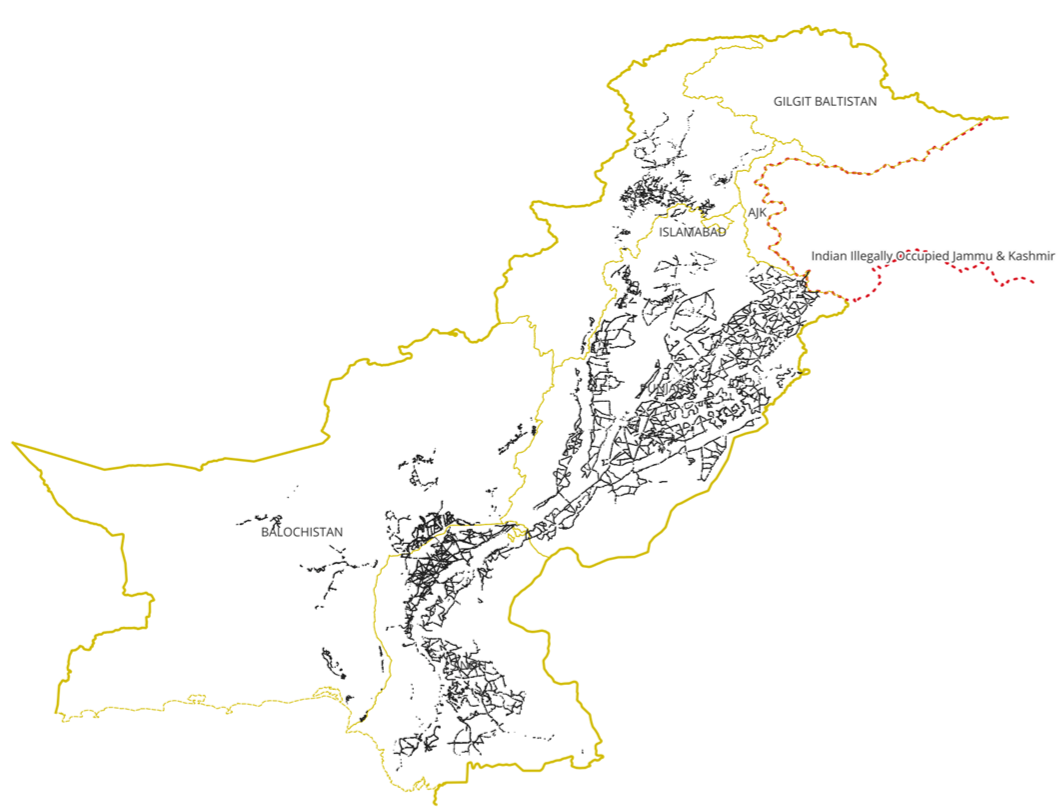
\includegraphics[width=0.85\columnwidth]{figs/Spatial_distribution.png}
\caption{Surveyed fields across the 79 districts of Pakistan, both seasons. The
protocol holds out entire districts, so calibration and evaluation regions are
geographically disjoint.}
\label{fig:spatial}
\end{figure}

Both seasons are steeply imbalanced, Wheat taking four fifths of Rabi and Rice over
half of Kharif, so macro-F1 is the primary metric. Classes below
1\% of a season are off-season rarities and are dropped, which removes Cotton,
Sorghum, Jantar, and Rice from Rabi. Five Rabi crops remain, with field counts Wheat
20{,}932 (79.2\%), Rapeseed 2{,}218 (8.4\%), Barseem 1{,}281 (4.8\%), Maize 1{,}134
(4.3\%), and Sugarcane 745 (2.8\%). Seven Kharif crops remain: Rice 32{,}477
(54.9\%), Cotton 12{,}179 (20.6\%), Sugarcane 7{,}487 (12.6\%), Maize 4{,}178
(7.1\%), Sorghum 1{,}189 (2.0\%), Jantar 887 (1.5\%), and Sesame 793 (1.3\%).

% ======================================================================
\section{Methodology}\label{sec:method}
% ======================================================================
The pipeline is summarised in Fig.~\ref{fig:flow}: each field's monthly Sentinel-2
series is classified by PhenoSSM, its out-of-fold scores are calibrated conformally
under a strict spatial protocol, and the backbone is optionally trained to tighten
the resulting prediction sets.

\begin{figure*}[t]
\centering
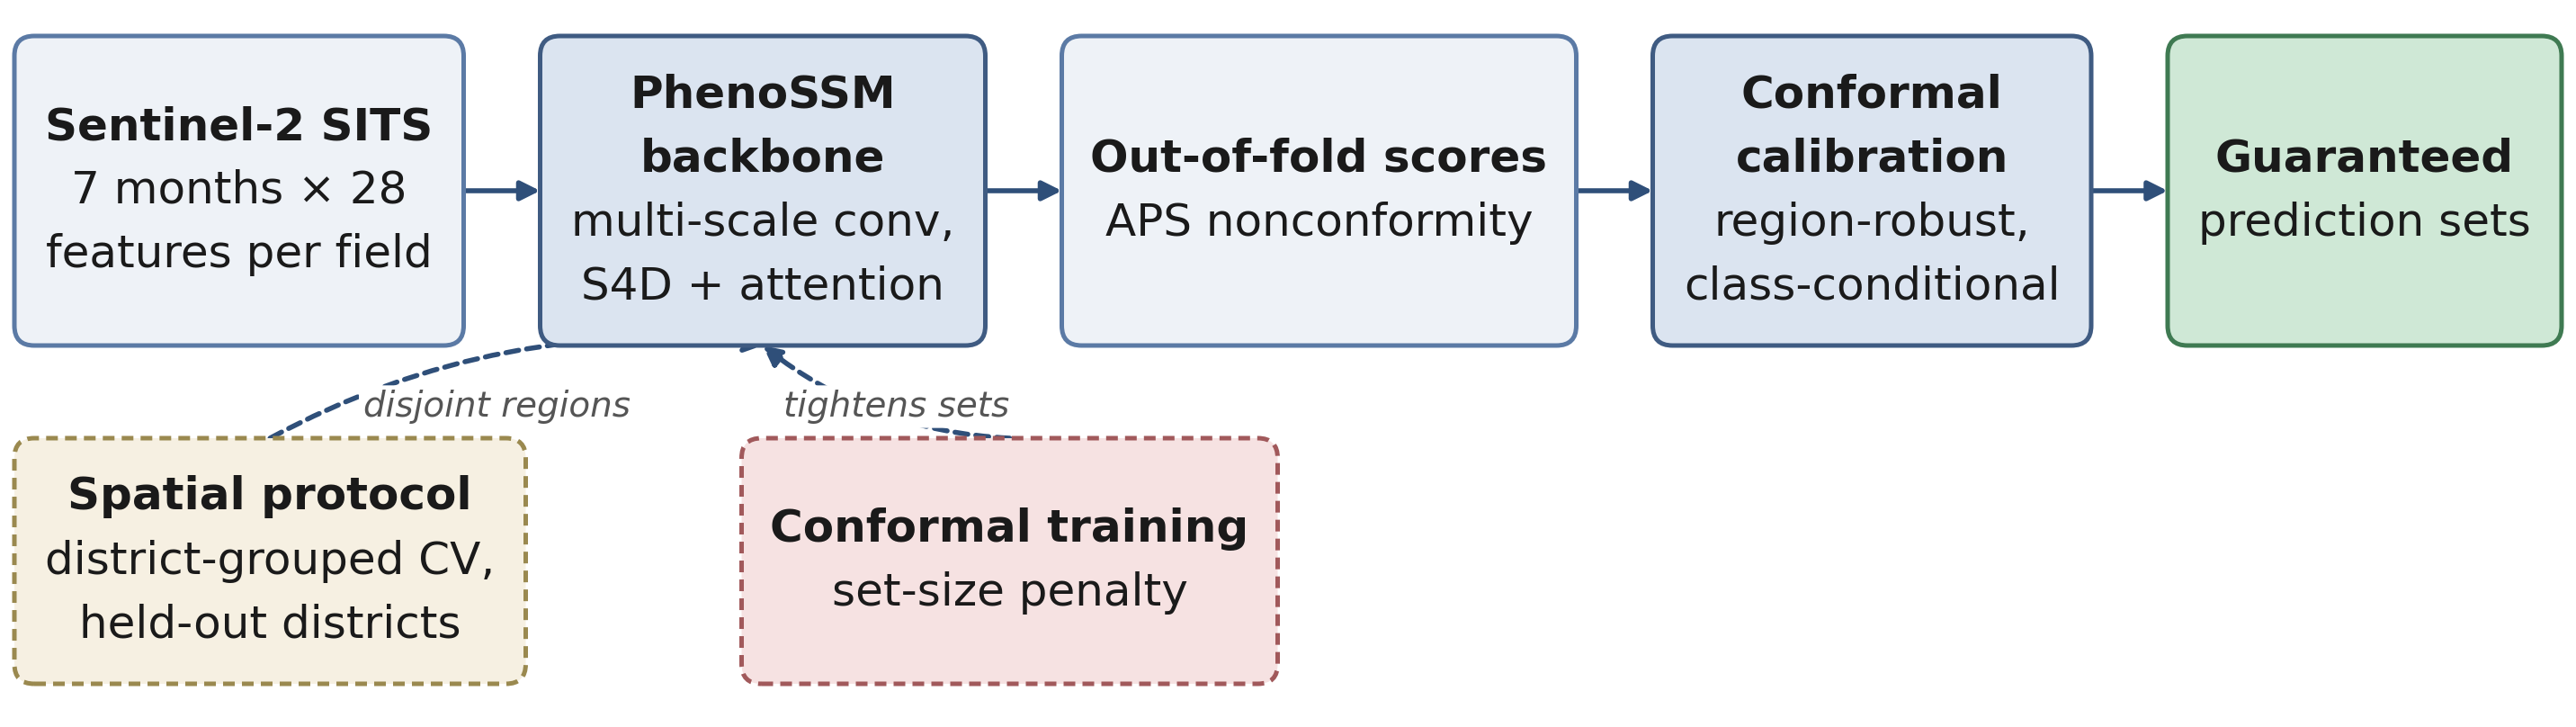
\includegraphics[width=\textwidth]{figs/method_flow.png}
\caption{Pipeline overview. Field-level Sentinel-2 series feed PhenoSSM, out-of-fold
scores are calibrated under the district-held-out protocol, and conformal training
feeds back to tighten the certified sets.}
\label{fig:flow}
\end{figure*}

PhenoSSM processes the per-field $T\times C$ sequence with a multi-scale
temporal-convolution front-end (kernels two, three, five), a diagonal state-space
backbone (S4D~\cite{gu2022s4d}), and a temporal-attention head (Fig.~\ref{fig:phenossm}).
Its components are accuracy-neutral over a plain S4D backbone, so it is a compact,
efficient default rather than an accuracy claim.

\begin{figure*}[t]
\centering
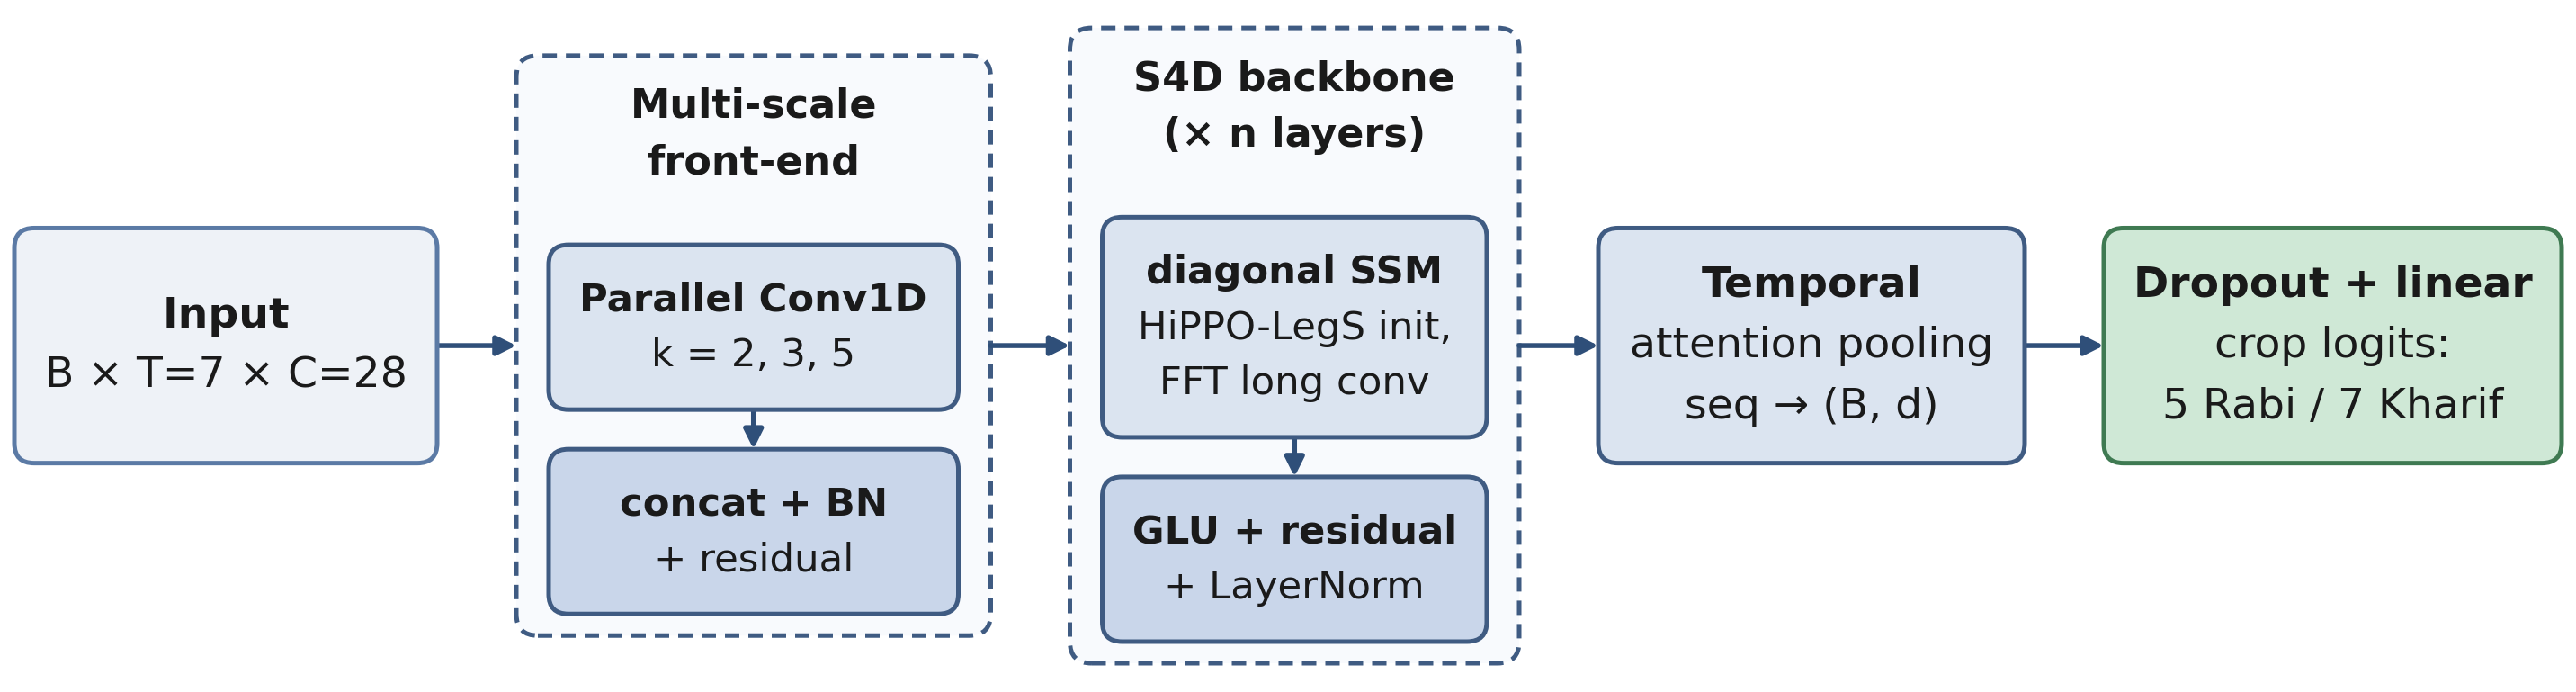
\includegraphics[width=\textwidth]{figs/phenossm_arch.png}
\caption{PhenoSSM. A multi-scale temporal-convolution front-end (kernels 2, 3, 5)
feeds stacked diagonal S4D blocks, pooled by temporal attention before a linear
classifier (147K parameters).}
\label{fig:phenossm}
\end{figure*}

Every field of a district stays within a single fold. District-grouped five-fold
cross-validation is paired with a test set of entirely held-out districts, and
normalisation is fit on the training fold alone.

Let $s(x,y)$ be a nonconformity score; adaptive prediction sets~\cite{romano2020aps}
are used. Given calibration scores from a region $\mathcal{C}$, the threshold is
$\hat q = \mathrm{Quantile}(1-\alpha;\,\{s(x_i,y_i)\}_{i\in\mathcal{C}})$ and the set
is $\Gamma(x)=\{y:s(x,y)\le\hat q\}$, valid under exchangeability, which geographic
deployment breaks. Four schemes are compared. Marginal uses one global $\hat q$ and
Mondrian one per crop. Region-robust calibrates $\hat q_d$ within each training
district and takes a conservative inter-district quantile,
\begin{equation}
\hat q_{\mathrm{RR}} = \mathrm{Quantile}\!\left(\tau;\ \{\hat q_d\}_{d\in\mathcal{D}}\right).
\end{equation}
Class-conditional region-robust applies that same construction within each crop,
$\hat q^{(c)}_{\mathrm{CRR}} = \mathrm{Quantile}(\tau;\ \{\hat q_{c,d}\}_{d\in\mathcal{D}_c})$.
It falls back to the pooled per-crop quantile, and then to the global one, for the
sparse (crop, district) cells the rare crops produce. This is an empirical,
group-based instance of distributionally robust conformal
prediction~\cite{cauchois2024robust}. Conditional coverage over arbitrary regions is
impossible~\cite{barber2023nonexchangeable}, so $\tau$ is a tunable safety margin,
selected on a disjoint pool of tuning splits.

Region-robust calibration certifies valid sets but does not make them small.
PhenoSSM is therefore trained to produce scores the conformal layer can certify
tightly, following conformal training~\cite{stutz2022conformal}. Each minibatch is
split into a calibration and a prediction part. A differentiable threshold $\hat q$
is taken at level $1-\alpha$ from the calibration true-class scores, and soft
prediction sets $E_{x,c}=\sigma((\hat q - s(x,c))/T)$ are formed on the prediction
part. A smooth size penalty is then added to the base loss,
\begin{equation}
\mathcal{L} = \mathcal{L}_{\mathrm{SCE}} + \lambda\,\mathbb{E}\Big[\max\big(0,\textstyle\sum_c E_{x,c}-\kappa\big)\Big],
\end{equation}
with temperature $T$, $\kappa{=}1$, and $\lambda{=}0.1$. The base loss keeps the true
class probable, so coverage holds, while the penalty shrinks the sets the deployed
conformal layer will certify, at unchanged training cost and identical inference.
Five losses are compared: cross-entropy, focal loss~\cite{lin2017focal}, logit
adjustment~\cite{menon2021logitadjust}, generalized cross-entropy~\cite{zhang2018gce},
and symmetric cross-entropy~\cite{wang2019sce}. Putative label noise is estimated with
an uncertainty-guided variant of confident learning~\cite{northcutt2021confident}, and
the per-class rates are model-derived diagnostics rather than truth.

% ======================================================================
\section{Experimental Setup}
% ======================================================================
Seven baselines are trained under an identical spatial protocol: Random Forest, TempCNN~\cite{pelletier2019tempcnn}, an LSTM, L-TAE~\cite{garnot2020ltae}, S4D~\cite{gu2022s4d}, MSTACNN (multi-scale attention CNN), and a temporal Transformer encoder (chosen over spatio-temporal architectures like TSViT~\cite{tarasiou2023tsvit}, which require a spatial axis absent in field-aggregated inputs). All models use Adam ($\text{lr}=10^{-3}$), batch size 256, up to 150 epochs, early stopping on validation macro-F1, and three seeds. Conformal coverage is measured over 25 held-out district splits, tuning $\tau$ on a disjoint pool of 25.Two further protocols probe distribution shifts. Leave-one-province-out calibrates outside a held-out province and evaluates inside it across all four provinces, reporting macro and worst-crop metrics for classes with $\ge 30$ fields. The phenology-shift test shifts the monthly window by $k$ months (with edge replication), calibrating on half the held-out districts and testing on the shifted remainder across 25 splits. Both protocols use the five-fold ensemble, as single-fold thresholds fail to transfer to ensemble probabilities. Significance against PhenoSSM is assessed per seed via McNemar's test with Holm correction. Experiments run on a single RTX 5060 GPU. Code, weights, and evaluation routines will be made publicly available\footnote{Repository URL provided in the camera-ready version.}.

% ======================================================================
\section{Results}
% ======================================================================
\subsection{Accuracy and the Optimism of Random Validation}\label{ssec:bench}
All eight backbones were trained under the spatial protocol with cross-entropy and
three seeds. Cross-validation macro-F1 spans .808 to .851 on Rabi and .688 to .767 on
Kharif. PhenoSSM (147K parameters) leads Rabi at every seed and beats every deep
baseline on the held-out test after Holm correction (median $p\le.006$). On Kharif it
sits within 0.015 of S4D, the Transformer, and MSTACNN, which the McNemar tests do not
separate at any seed (median $p$ of .35, .15, and .06), though it stays above L-TAE
and TempCNN. Accuracy is therefore saturated across architectures, and the reliability
results below ride on any backbone. The across-seed deviation is at most 0.013, while
the per-fold spatial spread of 0.02 to 0.05 reflects real between-region difficulty.
Random validation is measurably optimistic: under random folds PhenoSSM reaches 0.878
on Rabi and 0.827 on Kharif, against 0.851 and 0.757 under the spatial protocol, and
the fold-to-fold deviation collapses from near 0.02 to 0.005 on Kharif. That is the
accuracy analogue of the coverage optimism below.

\subsection{Training Objective and Label Noise}\label{ssec:loss}
Swapping the loss on PhenoSSM, symmetric cross-entropy is best and is the shipped
choice, at macro-F1 0.856 on Rabi and 0.778 on Kharif. The other four, cross-entropy,
focal loss, logit adjustment, and generalized cross-entropy, span 0.830 to 0.845 and
0.746 to 0.772. Only the noisier Kharif separates them, since the Rabi spread sits
inside a fold variance of 0.014 to 0.067. Long-tail losses do not help: focal loss and
logit adjustment up-weight hard rare examples, but those carry the most estimated
noise, so stressing them amplifies the bad labels. Relabel cleaning gave no held-out
gain either (0.826 to 0.825 on Rabi, 0.714 to 0.709 on Kharif), because it drags hard
rare-crop fields into the majority. A controlled test confirms the mechanism: with
symmetric noise added to the Kharif training labels, cross-entropy collapses from
0.754 to 0.364 macro-F1 at 30\% noise while symmetric cross-entropy holds at 0.749.

\subsection{The Geographic Coverage Gap}\label{ssec:geoshift}
This is the core result (Table~\ref{tab:conf}). Each field is scored by the
cross-validation fold that never trained on it, and the pool is then cut by district
into a calibration and an evaluation region. Under i.i.d.\ splits marginal conformal
is exact, which validates the implementation, and because both split types use the
same calibration and evaluation sizes the extra spread is geographic, not
finite-sample. Under shift the mean marginal coverage is roughly held at 0.89 in both
seasons, while its per-region standard deviation rises by more than an order of
magnitude. The target is missed in 24\% (Rabi) and 28\% (Kharif) of regions, and the
worst region falls to 0.77 and 0.68.

Two layers of the failure show in the per-crop columns. The region-robust threshold
cuts overall violations to 4\%, but it sets one value for the whole region, so on Rabi
the worst-covered crop reaches only 0.72 and mean per-crop coverage 0.87. Mondrian
conditions on the crop but not the region, lifting per-crop coverage yet losing
overall coverage (36\% violations on Rabi). Conditioning on both restores per-crop
coverage, raising the worst crop to 0.94 (Rabi) and 0.96 (Kharif), at a cost treated
in Section~\ref{ssec:rare}.

Region-robust calibration is the right tool here, not merely the simplest.
Importance-weighted conformal reweights calibration points by a domain-classifier
likelihood ratio~\cite{tibshirani2019covshift} and collapses under group shift.
Disjoint districts make the ratio degenerate, the effective sample falls to 6 to 9\%,
and coverage drops to 0.84 (Rabi) and 0.57 (Kharif), worse than plain marginal. The
inter-district quantile needs no density ratio at all. The gap is also not specific to
PhenoSSM. Across all eight backbones marginal conformal violates the target in 16 to
40\% of regions, and region-robust calibration drives violations to zero for every
deep model, with Random Forest reaching 12\% on Kharif. Coverage and set size both
rise with $\tau$, from 0.903 at 1.99 crops ($\tau{=}0.7$, Rabi) to 0.967 at 2.92
($\tau{=}0.95$), with the largest step between 0.9 and 0.95.

\begin{table}[t]\centering\caption{Conformal coverage over 25 held-out geographic
splits at the 90\% target ($\tau{=}0.9$), stock PhenoSSM. Cov.\ is overall coverage,
macro the mean per-crop coverage, w-crop the worst crop. Weighted is
importance-weighted conformal~\cite{tibshirani2019covshift}.}\label{tab:conf}
\footnotesize
\setlength{\tabcolsep}{3.5pt}
\begin{tabular}{lccccc}
\toprule
Scheme & Cov.\ (m$\pm$s) & Viol. & macro & w-crop & Size\\
\midrule
\multicolumn{6}{c}{\textit{Rabi (5 crops)}}\\
i.i.d.\ marginal      & .900$\pm$.003 & 0\%  & --   & --   & 1.95\\
marginal              & .893$\pm$.046 & 24\% & .795 & .626 & 1.94\\
weighted              & .841$\pm$.167 & 44\% & .752 & .594 & 1.77\\
Mondrian              & .880$\pm$.053 & 36\% & .870 & .830 & 2.47\\
region-robust         & .949$\pm$.031 & 4\%  & .868 & .718 & 2.47\\
class-region-robust   & .950$\pm$.023 & 0\%  & \textbf{.976} & \textbf{.943} & 4.42\\
\midrule
\multicolumn{6}{c}{\textit{Kharif (7 crops)}}\\
i.i.d.\ marginal      & .900$\pm$.002 & 0\%  & --   & --   & 2.94\\
marginal              & .899$\pm$.069 & 28\% & .902 & .795 & 2.99\\
weighted              & .574$\pm$.368 & 64\% & .643 & .504 & 1.80\\
Mondrian              & .893$\pm$.061 & 28\% & .892 & .864 & 2.67\\
region-robust         & .962$\pm$.028 & 4\%  & .944 & .880 & 3.65\\
class-region-robust   & .969$\pm$.018 & 0\%  & \textbf{.980} & \textbf{.962} & 5.32\\
\bottomrule
\end{tabular}\end{table}

\subsection{Per-Crop Coverage and the Long Tail}\label{ssec:rare}
Per-crop coverage is paid for in set size, and the bill falls on the crops the
guarantee is meant to protect (Fig.~\ref{fig:rare}). Averaged over all fields the
class-conditional region-robust sets hold 4.4 of five candidate crops on Rabi and 5.3
of seven on Kharif. Per true crop the picture is starker. The three rare Kharif crops,
Sesame, Jantar, and Sorghum, each under 1{,}200 fields, are covered at 0.98 with sets
of 5.3 to 5.5 of seven and almost never a single one. The rare Rabi crops reach 0.97
or better with 3.4 to 4.2 of five. A set that size rules out one or two crops and
names none, so it is reliable without supplying an answer.

Per-crop validity under shift is therefore met by abstaining. That is a property of
the problem rather than of this implementation, and it is what the limit noted in
Section~\ref{sec:method} looks like once a crop is both rare and spatially varied. Nor
is it a fallback artefact: the scheme forms a genuine inter-district quantile for
every crop, the rarest (Sesame, Jantar) drawing on six to nine districts. A deployer
needing an answer rather than a guarantee should read the region-robust row instead,
where Sesame and Jantar sit at 4.5 of seven with coverage near 0.92, and accept a
regional rather than per-crop guarantee.

\begin{figure}[t]
\centering
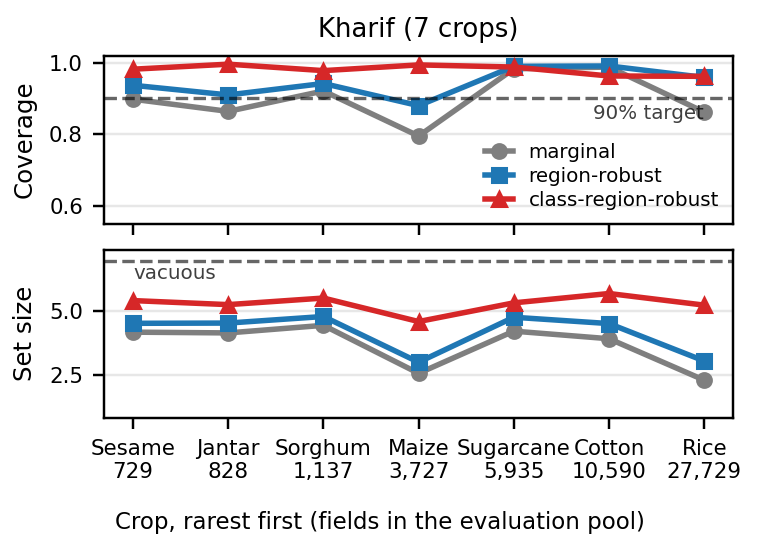
\includegraphics[width=\columnwidth]{figs/rare_crop_size.png}
\caption{The cost of per-crop validity on Kharif, crops ordered rarest first.
Class-conditional region-robust calibration (red) lifts every crop over the 90\%
target, and pays for it with sets near the vacuous ceiling of seven. Marginal (grey)
falls below target on Maize and Rice. Rabi behaves the same on a ceiling of five.}
\label{fig:rare}
\end{figure}

\subsection{Province Transfer and Phenology Shift}\label{ssec:transfer}
The district splits above hold out a random half of the districts. Two harder tests
ask whether the remedy survives a larger shift (Table~\ref{tab:transfer}).

The first holds out an entire province in turn, calibrating on every district outside
it. Pakistan's four provinces differ in agro-ecology, irrigation regime, and crop mix,
so this is a larger shift than a random district split. Marginal conformal degrades
further, and the worst province is severe: Balochistan falls to 0.76 on Rabi and 0.60
on Kharif, where its rice is covered at 0.39. Region-robust calibration at
$\tau{=}0.9$ lifts every Rabi province over the target but leaves Balochistan at 0.82
on Kharif, so the margin tuned on district splits is not enough at province scale.
Raising $\tau$ to 0.95 clears all four provinces at a modest cost in set size. The
scale of the expected shift has to be built into $\tau$.

The second test stands in for year-to-year variation, which a single survey year
cannot supply. The main year-to-year effect on a crop series is a phenological offset,
since sowing and harvest slide by weeks when the monsoon or a cold spell arrives off
schedule. The monthly window of the held-out test fields is therefore re-indexed by
$k$ months while calibration stays unshifted, as it would be from a previous, normal
year. Accuracy degrades steeply with the offset, but coverage does not collapse with
it. Region-robust calibration holds at or above the target through a one-month offset
in both seasons, and it does so by enlarging the sets. The conformal layer turns a
silent accuracy loss into a visible loss of precision, which is what a deployed map
needs. At two months the seasons part company: Kharif still holds at 0.98 by widening
to 4.0 and 4.4 crops, whereas Rabi drops to 0.88 and the guarantee fails. Why is not
established here, beyond Rabi's smaller crop pool leaving less room to absorb an
error. This is a simulation on a shifted copy of one year, not a second year of ground
truth. Its pool carries only 10 to 11 districts, so the $k{=}0$ row is the reference
for the rest of the column.

\begin{table}[t]\centering\caption{Two larger shifts at the 90\% target. Upper:
leave-one-province-out, mean over the four provinces and the worst one. Lower: the
phenology-shift stress test, calibration unshifted and the evaluation window
re-indexed by $k$ months. RR is region-robust.}\label{tab:transfer}
\footnotesize
\setlength{\tabcolsep}{3.5pt}
\begin{tabular}{lcccccc}
\toprule
 & \multicolumn{3}{c}{Rabi} & \multicolumn{3}{c}{Kharif}\\
Scheme & Cov. & worst & Size & Cov. & worst & Size\\
\midrule
\multicolumn{7}{c}{\textit{Leave-one-province-out}}\\
marginal            & .897 & .759 & 2.03 & .856 & .598 & 2.92\\
RR ($\tau{=}0.9$)   & .950 & .902 & 2.53 & .935 & .824 & 3.47\\
RR ($\tau{=}0.95$)  & .985 & .975 & 3.37 & .980 & .970 & 3.93\\
class-RR            & .957 & .877 & 4.64 & .945 & .822 & 5.14\\
\midrule
\multicolumn{7}{c}{\textit{Phenology shift, region-robust ($\tau{=}0.9$)}}\\
 & F1 & Cov. & Size & F1 & Cov. & Size\\
$k{=}{-}2$ months   & .430 & .881 & 3.62 & .560 & .982 & 3.98\\
$k{=}{-}1$          & .654 & .976 & 3.11 & .722 & .975 & 3.35\\
$k{=}0$             & .837 & .899 & 2.29 & .776 & .955 & 3.17\\
$k{=}{+}1$          & .701 & .960 & 2.91 & .701 & .964 & 3.48\\
$k{=}{+}2$          & .490 & .877 & 3.32 & .564 & .986 & 4.44\\
\bottomrule
\end{tabular}\end{table}

\subsection{Conformal-Efficiency-Aware Training}\label{ssec:conftr}
Tighter sets, not more coverage, are what is missing, so PhenoSSM is also trained with
the set-size penalty at $\lambda{=}0.1$. Accuracy is unchanged within fold variance
(CV macro-F1 0.859 Rabi, 0.780 Kharif), and per-region coverage becomes more uniform,
the Kharif worst region rising from 0.68 to 0.79. The sets also become more
informative, though the gain sits with the common crops. On Kharif the region-robust
set shrinks from 3.65 to 3.07 crops, singletons rise from 7.1 to 12.8\%, and macro and
worst-crop coverage reach 0.955 and 0.928. On Rabi the mean size is unchanged at 2.47,
with extra singletons (11.2 to 13.5\%) offset by a few larger sets. The
class-conditional sets tighten from 4.42 to 4.29 crops on Rabi and 5.32 to 4.92 on
Kharif, but their singleton rate stays at zero, so the rarest crops are unchanged. A
sweep of $\lambda\in\{0.05,0.1,0.2,0.5\}$ saturates: $\lambda{=}0.2$ lifts the Rabi
worst crop from 0.72 to 0.84 but erodes validity, and $\lambda{=}0.5$ costs Kharif
accuracy. Training for set size therefore moves the frontier up to the
representation's floor rather than removing it. For throughput, a temperature-scaled
five-fold ensemble reaches about 98\% accuracy at 80\% coverage, so the confidence
route automates the easy majority while the sets attach to the deferrals.

% ======================================================================
\section{Discussion and Limitations}
% ======================================================================
Three lessons carry beyond crops. The gap comes from spatial autocorrelation, not from
anything specific to crops, so other maps built the same way, such as land-cover or
forest-type, are likely to show it too. One country and one year cannot prove that, so
it stays a conjecture. The safety margin must match the size of the shift expected: a
$\tau$ tuned between neighbouring districts was too small for whole provinces. Both
calibration schemes need only a group label for each sample, so the same recipe fits
any setting where calibration and target data come from different groups, such as
different hospitals. Architecture matters least, since accuracy was saturated across
all eight backbones and the gap and its fix held for every one.

The limits are easy to state. All results come from one country and one cropping year,
so only spatial transfer was tested, and the phenology test of
Section~\ref{ssec:transfer} shifts a copy of that same year rather than replacing a
second season of ground truth. The numbers here should not be assumed to hold for
another country, year, or sensor, although the problem itself probably will appear
there too. Label noise was estimated by the model, not checked by hand, and $\lambda$
came from a coarse sweep. The rarest crops, under 60 test fields, remain hard. To
deploy, split the calibration data by region, fit one threshold per region, and use
the $\tau$ quantile of those thresholds rather than a single pooled one, taking 0.9
between neighbouring districts and 0.95 across agro-ecological zones. Report the worst
region's coverage next to the mean, and treat low-confidence outputs as advice rather
than as grounds for decisions such as subsidy payments.

% ======================================================================
\section{Conclusion}
% ======================================================================
This work identified and characterised the geographic coverage gap, the loss of
conditional coverage that appears when a conformal predictor calibrated in one region
is deployed in another. It holds across eight backbones, which makes it a property of
spatially structured geospatial learning rather than of any single model.
Region-robust calibration closes it for overall coverage and a class-conditional
variant closes it per crop, the latter only with near-vacuous sets for the rare
classes, which conformal-efficiency-aware training tightens no further than the
representation's floor. Holding out whole provinces showed the construction
transferring to a larger shift while its safety margin did not, so the margin has to
match the distance between calibration and deployment. This rests on one country and
one cropping year and covers spatial transfer alone. Because the mechanisms turn on
spatial structure and class imbalance, the same gap and remedies plausibly extend to
other spatially structured mapping tasks, which the released testbed is meant to let
the community test.

% ======================================================================
\section*{Acknowledgment}
% ======================================================================
The authors acknowledge funding support from the UK Research and Innovation (UKRI)
through Project APP47457, titled ``Super-efficient Sustainable Cooling Solution for
All Applications (S2Cool)'', under the Ayrton Challenge Program.

\bibliographystyle{IEEEtran}
\bibliography{references}
\end{document}
